\documentclass[8pt,a4paper]{report}
\usepackage[latin1]{inputenc}
\usepackage{amsmath}
\usepackage{amsfonts}
\usepackage{amssymb}
\usepackage{graphicx}
\usepackage{hyperref}
\usepackage{multicol}
\usepackage[margin=0.4in]{geometry}
\usepackage{karnaugh-map}
\usepackage{amsthm}
\usepackage{mathtools}
\usepackage{listings}
\newcommand{\myvec}[1]{\ensuremath{\begin{pmatrix}#1\end{pmatrix}}}
\let\vec\mathbf
\begin{document}

\vspace{15mm}
\centering \Large \textbf{ASSIGNMENT- OPTIMIZATION}
\vspace{15mm}
\begin{multicols}{2}


\raggedright \Large \textbf{Contents} \vspace{2mm}
\begin{itemize}
\raggedright \item Problem \item Solution\item Construction
\end{itemize}\vspace {5mm}
 

\raggedright \Large \textbf{Problem:} \vspace{2mm}
	\\ Find the shortest distance of the point (0,c) from the parabola $y = x^2$ where $0\le c \le 5$.\vspace{4mm}
\\\raggedright\Large \textbf{Solution:} \vspace{2mm}
 \\ \raggedright \textbf{Optimization}
\\ \raggedright Any conic of the form 
	\\ \centering $\vec{x^{\top}}\vec{V}\vec{x} + 2\vec{u^{\top}}\vec{x} + f = 0$ 
\\ \raggedright can be written as
	\\ \centering $\vec{x^{\top}}\vec{A}\vec{x} = 0$ 
	\\ where $\vec{A} = \myvec{\vec{V}&\vec{u}\\\vec{u^{\top}}&f}$, $\vec{x} =\myvec{x\\y\\1}$
	\\ \raggedright The distance from point $\vec{p} = \myvec{0\\c}$ to the point 'x' on parabola is $\|\vec{x}-\vec{p}\|^2$
\begin{gather*}
	\implies \vec{x^{\top}}\vec{x} - 2\vec{p^{\top}}\vec{x} + \|\vec{p}\|^2
\end{gather*}
	\\ \raggedright The above equation can be written as \\\centering $\vec{x^{\top}}\vec{C}\vec{x}$
	\\ \raggedright where $\vec{C} = \myvec{\vec{I}&-\vec{p}\\ -\vec{p^{\top}}& \|\vec{p}\|^2}$, $\vec{x} = \myvec{x\\y\\1}$
	\\ \raggedright The shortest distance is given by,
	\\ \centering min $\vec{x^{\top}}\vec{C}\vec{x}$
	\\ \raggedright such that,          \\ \centering $\vec{x^{\top}}\vec{A}\vec{x} = 0$
	\\ \raggedright Using SDR(Semi Definite Relaxation), it can be rewritten as 
	\\ \centering min $Tr\myvec{\vec{C}\vec{X}}$
	\\ \raggedright Suc that, 
	\\ \centering $ Tr\myvec{\vec{A}\vec{X}} =0,$
	\\ \centering $\vec{X}\ge0$
	\\ \raggedright Here , $\vec{X}$ is a  $3\times3$ matrix of variables where
	\\ \centering $ \vec{X} = \vec{x}\vec{x^{\top}}$
\centering 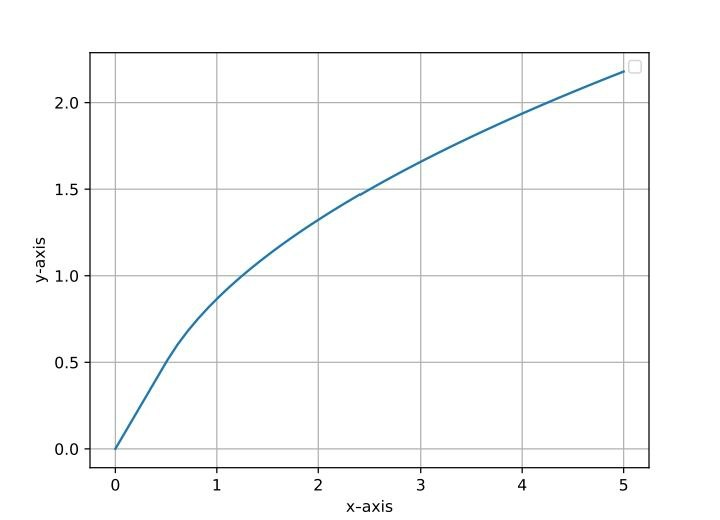
\includegraphics[width=1\columnwidth]{opt.jpg}
\end{multicols}
\end{document}
